\chapter{Design and Implementation}
\section{Chapter Overview}
This chapter will introduce the modules developed in this project including data collection, natural language data processing, text classification, named entity recognition, information extraction and other modules, and introduce the exploration of data integration in this project.
\begin{figure}[H]
\centering 
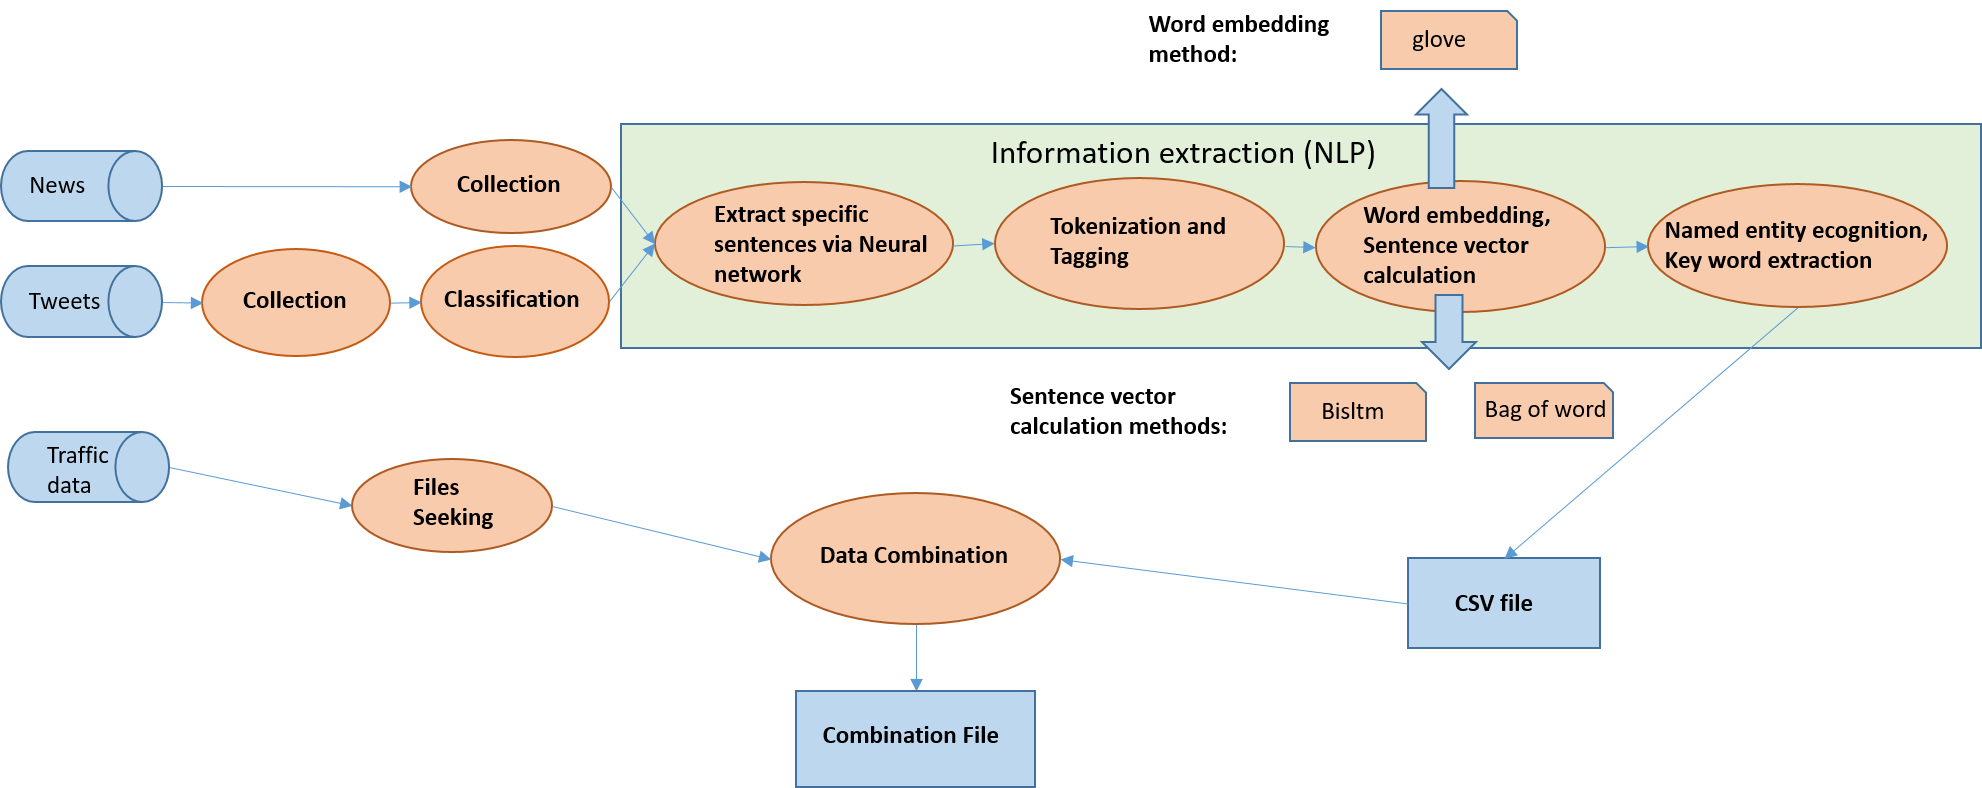
\includegraphics[width=1\textwidth]{data-flow.png}
\caption{The structure of the project}
\end{figure}
Taking the BBC News website as the data source as an example, the process of the entire project is shown in Figure 3.1. Natural language data is obtained from the BBC website, and then sentence classification is performed through the neural network to find the sentence to be extracted, and then pick the selected sentence to undergo a series of preprocessing and finally information extraction. Simultaneously, according to the geographic location information extracted from the information, the google map API is used to obtain the latitude and longitude coordinates, and a CSV file is generated. In order to combine the data in the CSV file with the related sensor data, an algorithm is needed to find the corresponding excel files containing sensor data based on the latitude and longitude information in the CSV file, and then use the data combination algorithm to combine the CSV data with the sensor data, generate the final CSV file.
\section{Tools Used}
\subsection{Programming Language}
\subsubsection{Python}
Python is an high-level, interpreted, general-purpose programming language.This language is created by Guido van Rossum and first released in 1991, Python's design philosophy emphasizes code readability with its notable use of significant whitespace. Its language constructs and object-oriented approach aim to help programmers write clear, logical code for small and large-scale projects. The reason for choosing python as the development language is that this project involves machine learning, natural language processing, data processing and other fields. Among many programming languages, Python is commonly used in machine learning projects and artificial intelligence projects with the help of libraries like TensorFlow, Keras, Pytorch and Scikit-learn. As a scripting language with modular architecture, simple syntax and rich text processing tools, Python is often used for natural language processing.[167]
\subsection{Database}
\subsection{Softwares}
\subsection{APIs}
\section{Data Collection}

% Local Variables: 
% mode: latex
% TeX-master: "report"
% End: 
